\documentclass[sigconf,nonacm]{acmart}
\usepackage{subcaption}
\graphicspath{{figures/}{../part1/figures/}}

\begin{document}

\title{COS 487 / 587 Course Project Part 2: IR Rangers}


\author{Esther Greene}
\affiliation{%
  \institution{University of Southern Maine}
  \city{Portland}
  \state{Maine}
  \country{USA}}
\email{esther.greene@maine.edu}

\author{Courtney Jackson}
\affiliation{%
  \institution{University of Southern Maine}
  \city{Portland}
  \state{Maine}
  \country{USA}}
\email{courtney.jackson@maine.edu}

\author{Nathaniel Serrano}
\affiliation{%
  \institution{University of Southern Maine}
  \city{Portland}
  \state{Maine}
  \country{USA}}
\email{nathaniel.serrano@maine.edu}

\begin{abstract}
% TODO rewrite once results are final. Points to hit:
% - continuation of Part 1: BM25 baseline vs. learned sparse (SPLADE) and dense (MiniLM) retrieval
% - SPLADE best single model: paper nDCG@5 0.631 vs 0.514 for BM25 (+23%)
% - Dense beats BM25 on papers but not on paragraphs
% - fine-tuning on Train gave no significant gain for either neural model
% - RRF of all three is significantly best: paper nDCG@5 0.655 (+27%), paragraph 0.489 (+18%)
% - analysis: neural models bridge paraphrase but still fall for shared vocabulary across fields
\end{abstract}

\keywords{information retrieval, BM25, SPLADE, dense retrieval,
rank fusion, scientific document retrieval, passage retrieval}

\maketitle

%======================================================================
\section{Introduction}
% TODO para 1: Part 1 recap in 2-3 sentences: BM25 beat TF-IDF, but
%   failed on hard queries that paraphrase terminology (vocabulary mismatch).
%   That motivates Part 2.
% TODO para 2: copy the collection description from Part 1 (34,308 papers,
%   2,275,574 paragraphs, noisy extraction) -- reuse as is.
% TODO para 3: copy the tasks / query sets / grading-scale paragraph from Part 1.
% TODO para 4: what's new: SPLADE and a dense bi-encoder, each zero-shot and
%   fine-tuned on Train; MaxP for papers; RRF fusion. Headline results.
The volume of scientific literature makes finding relevant work increasingly 
difficult, both at the level of whole papers and of the specific passages 
that answer a question. In the first phase of this project, we built a retrieval 
system for arXiv papers and paragraphs\footnote{Code: \url{https://github.com/esthergreene/IR-Rangers}} 
using two term-matching models, and found that BM25 significantly outperformed 
TF-IDF on both tasks. Our analysis also exposed the limits of exact term matching: 
hard queries that paraphrase technical terminology in general language, for 
example asking about ``wrist-worn optical sensors'' rather than PPG. share few 
terms with the document that answer them, and BM25 often failed on them, especially 
for paragraphs.

This paper describes the second phase, in which we add two neural retrieval models 
intended to bridge this vocabulary gap: a learned sparse model, SPLADE~\cite{formal2021splade}, 
which represents text as weights over vobcablulary terms, including related terms the 
text does not contain, and a dense bi-encoder~\cite{reimers2019sentence}, which 
represents text as a single embedding vector. We evaluate each model both as released 
and after fine-tuning on our Train queries, rank papers by their best-scoring 
paragraph~\cite{dai2019deeper}, and combine all three models with reciprocal rank 
fusion~\cite{cormack2009reciprocal}. BM25, our best model from part 1, serves as the 
baseline throughout.

The test collection consists of 34,308 arXiv papers published in August and September 2024. 
Each paper is provided both as raw HTML scraped from the ar5iv website and as a 
processed JSON file containing its identifier, title, abstract, and paragraphs. 
Because the JSON files were produced with rule-based extraction, they contain noise 
such as leftover \LaTeX{} markup and merged words, and display equations are missing 
altogether. In total, the collection contains 2,275,574 paragraphs, an average 
of about 66 per paper.

We address two tasks over this collection: \emph{paper retrieval}, which returns 
papers identified by their arXiv ID, and \emph{paragraph retrieval}, which returns 
individual paragraphs. For each query, systems return their top 100 results. Three 
query sets are provided: Train (2,000 queries), Study (250 queries with relevance 
judgements, which we use for all analysis in this paper), and Test (250 queries 
whose judgments are withheld). Each set contains 30\% easy, 50\% medium, and 25\% 
hard queries. Relevance is graded on a three-point scale: a document that fully 
addresses the query is relevant (2), one that provides useful information without 
fully addressing it is partially relevant (1), and any document not in the judgments 
is considered non-relevant.

SPLADE is the most effective single model on both tasks. On papers it improves nDCG@5 
over BM25 from 0.514 to 0.631; on paragraphs its advantage is smaller and not significant. 
The dense model outperforms BM25 on papers but not on paragraphs, and fine-tuning did 
not significantly improve either neural model. Fusing all three models gives the best 
results, with nDCG of 0.701 on papers and 0.550 on paragraphs, significantly above both 
BM25 and SPLADE alone. Our analysis shows that the neural models retrieve paragraphs 
that paraphrase the query, but still rank highly paragraphs that share the query's 
vobcabulary in an unrelated field.

\section{Methodology}
\label{sec:method}
% TODO overview paragraph: one pipeline, three first-stage retrievers
%   (BM25, SPLADE, dense), paragraph-level neural indexes, papers via MaxP,
%   optional RRF fusion.
Our system retrieves with three first-stage models that share the query 
sets, run format, and evaluation pipeline. BM25 (Section~\ref{sec:bm25}) 
searches inverted indexes over separately preprocessed paper and paragraph 
collections, as in Part~1. The two neural models, SPLADE (Section~\ref{sec:splade}) 
and a dense bi-encoder (Section~\ref{sec:dense}), receive more lightly preprocessed 
text (Section~\ref{sec:preprocessing}) and index paragraphs only. Both start from 
publically released checkpoints, which we evaluate as released and after fine-tuning 
on Train queries (Section~\ref{sec:training-data}). Because the neural indexes contain 
only paragraphs, papers are ranked from their paragraphs' scores (Section~\ref{sec:maxp}). 
Finally, runs from different models can be combined with reciprocal rank fusion 
(Section~\ref{sec:rrf}). Section~\ref{sec:eval} describes our evaluation setup.

\subsection{Preprocessing}
\label{sec:preprocessing}
% TODO condensed Part 1 text for BM25 (math removal, Snowball stemming, etc.)
%   + the collection-statistics table (tab:cleaning) if space allows.
% TODO neural input (config/preprocessing_neural.yaml): only cleaning --
%   inline math, URLs and citation markers removed; no stemming or stopword
%   removal, since the models use their own WordPiece tokenizers.
%   Mention the max input length / truncation if relevant.
BM25 and the neural models receive differently preprocessed text, because they 
match text in different ways.

For BM25, we keep the Part~1 pipeline unchanged. Inline mathematics, remaining 
\LaTeX{} commands, URLs, and numeric citation markers are removed; text is 
lowercased and split into alphanumeric tokens; tokens shorter than two characters 
or consisting only of digits are discarded; stopwords are removed using NLTK's English 
list~\cite{bird2009nltk}, extended with terms common in scientific writing such as ``et'', 
``al'', and ``fig''; and the remaining tokens are reduced with the Snowball 
stemmer~\cite{porter2001snowball}. Cleaning reduces the paragraph collection from 
168.0 to 114.9 million tokens (31.6\%) and leaves 8,389 paragraphs, almost all 
standalone formulas, empty. These are excluded, leaving 2,267,185 indexed paragraphs. 
Both encoders trucate their input at 256 WordPiece tokens.

\subsection{BM25 Baseline}
\label{sec:bm25}
% KEEP from Part 1: scoring function (equation), vectorized implementation,
%   and tuning on Train (k1 = 4.0, b = 0.75 for papers; paragraph values).
%   Cut TF-IDF entirely. The held-out tuning table can become one sentence.
% Reuse the Part 1 heatmap figure (bm25_tuning_paper_full.pdf,
%   bm25_tuning_paragraph_full.pdf) -- found via \graphicspath.
Our baseline is the BM25 model from Part~1, unchanged. It scores a document 
$d$ for a query $q$ as 
\begin{equation}
  \mathrm{score}(q,d) = \sum_{t \in q} \mathit{idf}_t \cdot
    \frac{\mathit{tf}_{t,d}\,(k_1 + 1)}
         {\mathit{tf}_{t,d} + k_1 \bigl(1 - b + b\,L_d / L_{\mathit{avg}}\bigr)},
  \label{eq:bm25}
\end{equation}
\begin{equation}
  \mathit{idf}_t = \ln\!\left(1 + \frac{N - \mathit{df}_t + 0.5}{\mathit{df}_t + 0.5}\right),
  \label{eq:idf}
\end{equation}
where $N$ is the number of documents, $\mathit{df}_t$ the number containing term 
$t$, $\mathit{tf}_{t,d}$ the occurrences of $t$ in $d$, and $L_d$ and $L_{\mathit{avg}}$ 
the length of $d$ and the average length, in tokens. This is the ``Lucene (accurate)'' 
variant of Kamphuis et al.~\cite{kamphuis2020bm25}, whose IDF remains positive for 
terms that occur in more than half of the documents. The parameter $k_1$ controls how 
quickly repeated occurrences of a term saturate, and $b$ how strongly scores are 
normalized by document length. Scoring is term-at-a-time over the postings of the query 
terms, vectorized with NumPy.

We tuned $k_1$ and $b$ separately for each collection by grid search on 1,600 Train 
queries, selecting the setting with the highest nDCG@5 (Figure~\ref{fig:tuning}). The 
selected settings, $k_1 = 4.0$, $b = 0.75$ for papers and $k_1 = 0.4$, $b = 0.9$ for 
paragraphs, also outperformed both the textbook values ($k_1 = 1.2$, $b = 0.75$)~\cite{manning2008irbook} 
and Anserini's defaults ($k_1 = 0.9$, $b = 0.4$)~\cite{yang2017anserini} on the remaining 
400 Train queries (nDCG@5 of 0.473 vs.\ 0.454 and 0.436 on papers, and 0.371 vs.\ 0.354 
and 0.344 on paragraphs). The tenfold difference in $k_1$ reflects document length: 
in a paper averaging 3,361 tokens, repeated occurrences of a term indicate its topic, 
whereas paragraphs, with a median of 40 tokens, rarely repeat a term, so whether a 
term occurs at all matters more.

\begin{figure}[t]
  \centering
  \begin{subfigure}{\columnwidth}
    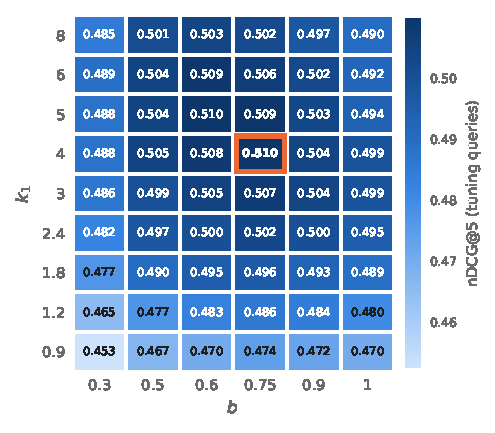
\includegraphics[width=\columnwidth]{bm25_tuning_paper_full.pdf}
    \caption{Papers.}
    \label{fig:tuning-paper}
  \end{subfigure}

  \vspace{0.5em}
  \begin{subfigure}{\columnwidth}
    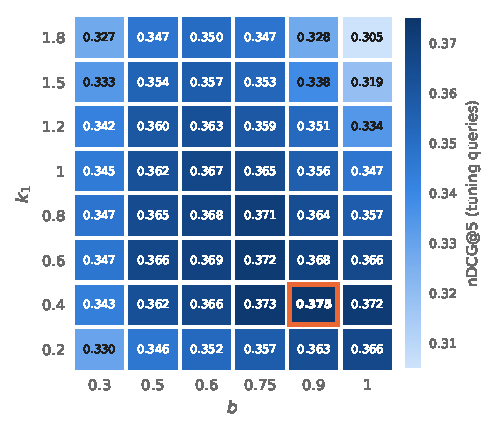
\includegraphics[width=\columnwidth]{bm25_tuning_paragraph_full.pdf}
    \caption{Paragraphs.}
    \label{fig:tuning-paragraph}
  \end{subfigure}
  \caption{BM25 nDCG@5 on 1,600 Train tuning queries. Outlined cells
    mark the selected settings.}
  \label{fig:tuning}
\end{figure}



\subsection{Training Data}
\label{sec:training-data}
% TODO (scripts/build_training_data.py; confirm the flags actually used):
% - only Train queries; split into train / validation by query (val fraction 0.1)
% - positives: judged paragraphs with grade >= 1 (confirm 1 vs 2)
% - hard negatives: judged-0 paragraphs, then paragraphs sampled from BM25's
%   ranking after skipping the top 20 (to avoid unjudged relevant ones);
%   30 per query, seeded
% - one (query, positive, negative) triple per judged positive, cycling negatives
% - leakage check: validation queries are disjoint from training queries; an
%   earlier version with 160 of 200 validation queries also in training gave an
%   inflated +9.65% that disappeared once fixed (1-2 sentences)
We fine-tune both neural models on Train queries only; Study and Test queries are 
never used for training or model selection. The 2,000 Train queries are split 
by query into 1,800 training and 200 validation queries, stratified by difficulty 
so that both sets keep the 30/50/20 mix of easy, medium, and hard queries, and no 
validation query appears in training. Every paragraph judged relevant or partially 
relevant serves as a positive, giving 5,138 positives for the training queries and 
582 for the validation queries, about 2.9 per query.

The Train judgments contain no non-relevant (grade 0) paragraphs, so negatives must 
be mined. We use BM25 hard negatives: unjudged paragraphs that BM25 retrieves for the 
query, which share vocabulary and topic with it and are therefore more informative 
than random paragraphs. Because judgments are incomplete, an unjudged paragraph near 
the top of BM25's ranking is often relevant, so we skip BM25's top 20 results and 
sample 30 negatives per query at random from ranks 21--100, with a fixed seed per query. 
Random sampling gives each query a mix of close and easier negatives rather than only 
the hardest ones. Each training example is a (query, positive, negative) triple, one 
per positive, cycling through the query's negatives. Both models are trained with a 
contrastive loss in which each query's positive must outscore its own hard negative 
as well as the positives and negatives of the other queries in the batch (Sections~\ref{sec:splade} 
and~\ref{sec:dense}).

Both models select their best checkpoint by nDCG@10 on the validation queries. Encoding 
all 2.28 million paragraphs at every evaluation would take 30 to 60 minutes (Section~\ref{sec:efficiency}), 
so validation instead ranks a fixed sample of the collection: every validation positive, 
the top 100 BM25 results for each validation query, and 10,000 random paragraphs. Scores 
on this sample are used only to compare checkpoints, not to report effectiveness.

\subsection{Learned Sparse Retrieval}
\label{sec:splade}
% TODO: SPLADE \cite{formal2021splade}: MLM head -> log-saturated ReLU,
%   max-pooled weights over the vocabulary; query and document are sparse
%   vectors, scored by dot product. Start from naver/splade-cocondenser-selfdistil
%   \cite{formal2022distillation}, which is also the zero-shot model.
% TODO fine-tuning: SparseMultipleNegativesRankingLoss (in-batch + hard negative)
%   + FLOPS regularization \cite{paria2020minimizing}; batch 32, lr 1e-5,
%   up to 3 epochs, eval every 50 steps, early stopping (patience 3) on
%   validation nDCG@10. Confirm run2's actual values.
% TODO index: paragraph vectors stored as a sparse matrix (.npz), searched
%   by sparse matrix-vector product.

\subsection{Dense Retrieval}
\label{sec:dense}
% TODO: bi-encoder all-MiniLM-L6-v2 \cite{wang2020minilm, reimers2019sentence},
%   384-dim mean-pooled embeddings, cosine / inner product.
% TODO fine-tuning: MultipleNegativesRankingLoss, batch 32, lr 2e-5, up to 5 epochs,
%   same early stopping. Confirm run1's actual values.
% TODO index: exact inner-product FAISS index \cite{johnson2019billion} (confirm
%   flat vs. approximate) over all 2.28M paragraphs.

\subsection{Paper Ranking}
\label{sec:maxp}
% TODO: neural models index paragraphs only. Each paper is scored by its
%   best paragraph (MaxP, \cite{dai2019deeper}) among the top 2,000 retrieved
%   paragraphs; keep the top 100 papers. BM25 papers still use the Part 1
%   paper index. Note why 2,000 (enough to fill 100 distinct papers).

\subsection{Rank Fusion}
\label{sec:rrf}
BM25, SPLADE, and the dense model match queries to documents in different ways, 
through exact terms, weighted and expanded terms, and a single embedding, so their 
errors may differ as well. To test whether they complement each other, we combine 
their rankings with reciprocal rank fusion (RRF)~\cite{cormack2009reciprocal}, 
which scores each document by its rank in each run:
\begin{equation}
  \mathrm{RRF}(d) = \sum_{m \in M} \frac{1}{k + \mathrm{rank}_m(d)},
  \qquad k = 60,
  \label{eq:rrf}
\end{equation}
where $M$ is the set of fused runs and $\mathrm{rank}_m(d)$ the rank of $d$ in 
run $m$; a document absent from a run contributes nothing for that run. RRF uses 
only ranks, so it needs no normalization of the models' differently scaled 
scores, and the constant $k$ limits how much a single top rank can dominate. We 
use the standard $k = 60$ without tuning. We fuse the top-100 runs of BM25 and 
SPLADE, and of all three models, separately for each collection, and keep the 
top 100 fused results per query. For papers, the BM25 paper run is fused with 
the neural models' MaxP paper runs. Fusion is evaluated on Study queries only 
and is not among our submitted Test runs.

\subsection{Evaluation Setup}
\label{sec:eval}
% KEEP Part 1 text: nDCG equation, MRR, P@k, lenient vs strict, 238 queries
%   for strict, two-sided paired t-test p < 0.05 with ranx.
% ADD: Recall@100.
% REVISE the comparison list: all pairs of BM25 / Dense / SPLADE;
%   zero-shot vs fine-tuned for each neural model; RRF vs its components.
% REVISE query-set roles: Train for BM25 tuning and neural training/validation;
%   Study for all results; Test for submitted runs and annotation.
We evaluate each run's top 100 results with six metrics: nDCG, nDCG@5, MRR, 
P@5, P@10, and Recall@100 , computed with ranx~\cite{bassani2022ranx}. For a 
ranking with relevance grades 
$\mathit{rel}_i \in \{0, 1, 2\}$ at ranks $i = 1, 2, \dots$,
\begin{equation}
  \mathrm{DCG@}k = \sum_{i=1}^{k} \frac{\mathit{rel}_i}{\log_2(i + 1)},
  \qquad
  \mathrm{nDCG@}k = \frac{\mathrm{DCG@}k}{\mathrm{IDCG@}k},
  \label{eq:ndcg}
\end{equation}
where $\mathrm{IDCG@}k$ is the DCG of an ideal ranking of the judged 
documents~\cite{jarvelin2002cumulated}; nDCG without a cutoff uses the full top 100. 
MRR is the mean over queries of $1/r$, where $r$ is the rank of the first relevant 
document (0 if none is retrieved), P@$k$ is the fraction of the top $k$ documents 
that are relevant, and Recall@100 is the fraction of a query's relevant documents 
that appear in the top 100. Recall@100 is new in this phase: it measures how much 
a model could contribute to fusion or to a later reranking stage, beyond its top 
ranks. Documents absent from the judgments count as non-relevant.

nDCG uses the relevance grades directly as gains. For MRR, P@$k$, and Recall@100, 
documents of grade 1 or 2 count as relevant. We also report strict MRR and P@5, in 
which only grade-2 documents count; queries without a grade-2 document are excluded 
from these, so they are averaged over 238 of the 250 Study queries.

We test differences between runs with a two-sided paired Student's t-test over 
queries at $p < 0.05$, using ranx, between every pair of runs in a table: BM25, 
SPLADE, and the dense model; the zero-shot and fine-tuned version of each neural 
model; and each fused run against BM25, SPLADE, and the other fused run. We do not 
correct for multiple comparisons, so with many tests some individual significant 
differences may be chance; we therefore emphasize differences that are consistent 
across metrics and collections.

The three query sets serve distinct purposes. Train queries are used for tuning 
BM25 (Section~\ref{sec:bm25}) and for training the neural models and selecting their 
checkpoints (Section~\ref{sec:training-data}). Study queries are used for all reported 
results, and the Test queries, whose judgments are withheld, for our submitted runs 
and manual annotation (Section~\ref{sec:annotation}).


\section{Evaluation Results}
\label{sec:results}

\subsection{Training}
\label{sec:training}
\begin{figure}[t]
  \centering
  \begin{subfigure}{\columnwidth}
    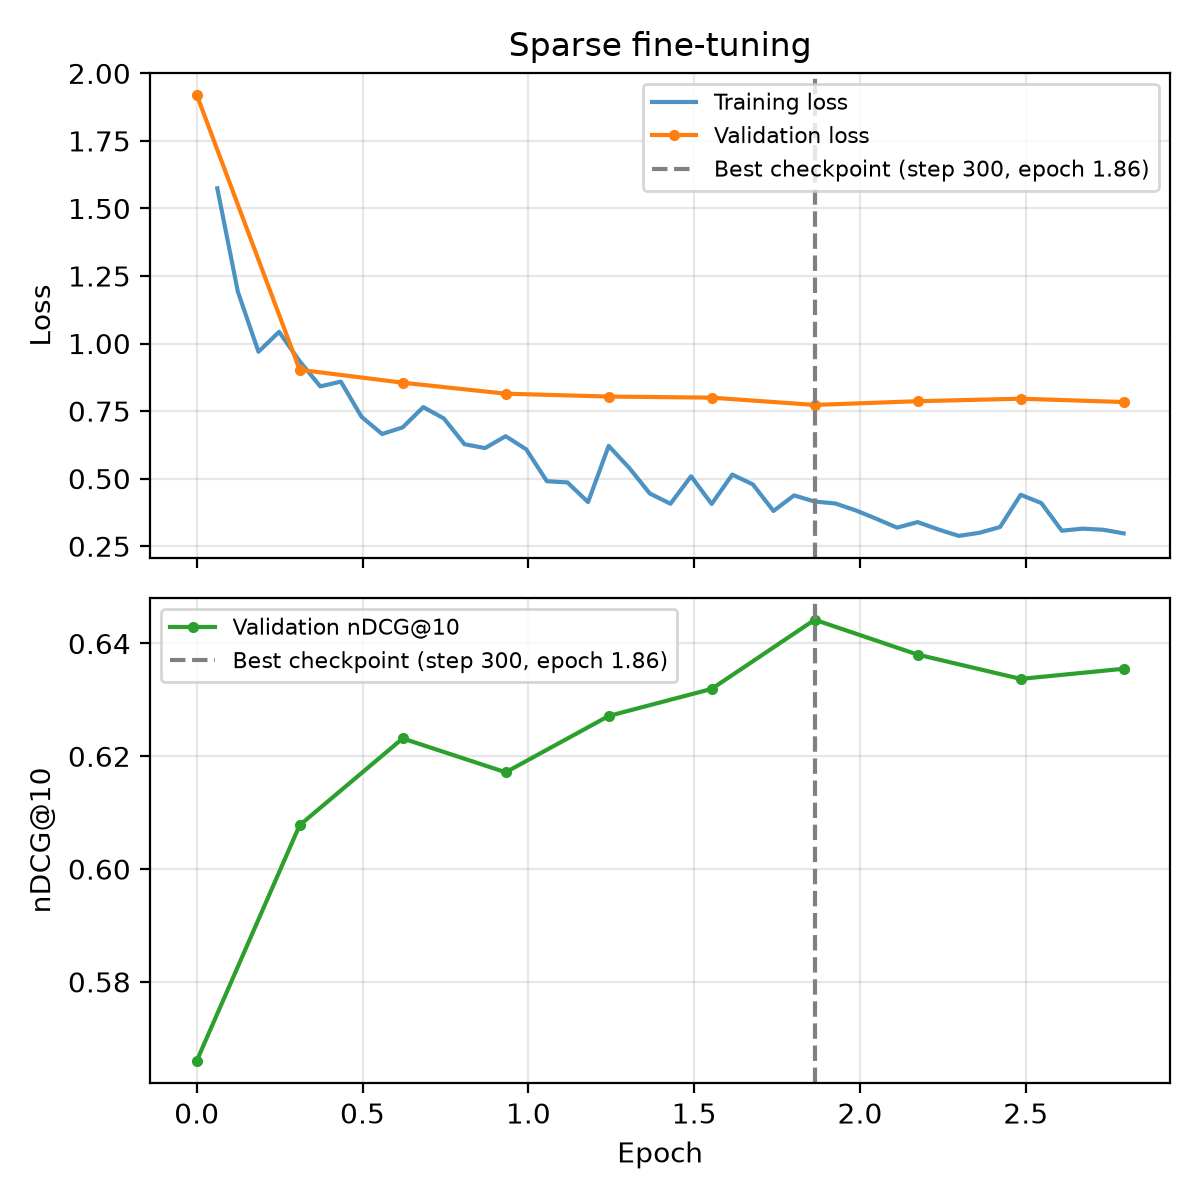
\includegraphics[width=\linewidth]{training_sparse_run2.png}
    \caption{SPLADE.}
  \end{subfigure}
  \begin{subfigure}{\columnwidth}
    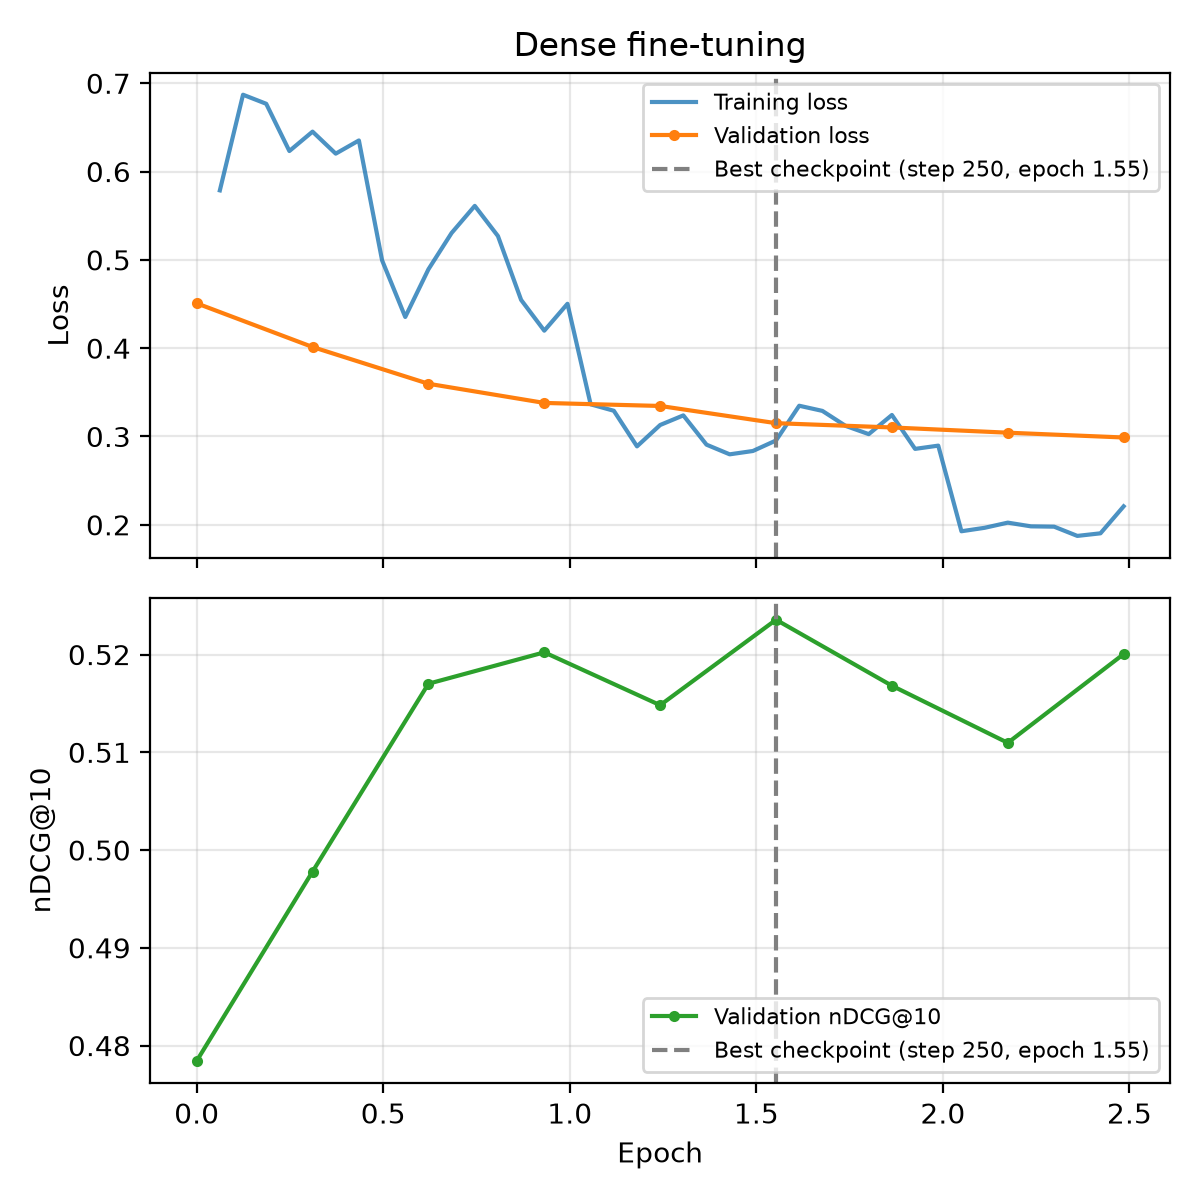
\includegraphics[width=\linewidth]{training_dense_run1.png}
    \caption{Dense (MiniLM).}
  \end{subfigure}
  \caption{Training and validation loss. % TODO: mark the selected checkpoint
  }
  \label{fig:training}
\end{figure}
% TODO describe curves: when val loss flattens, where early stopping picked
%   the best checkpoint, any overfitting gap.

\subsection{Effectiveness}
\label{sec:effectiveness}
\begin{table*}[t]
  \caption{Effectiveness on the 250 Study queries. Strict metrics count only
    grade-2 documents (238 queries). Superscripts mark a significant
    improvement over the model with that letter (paired t-test, $p < 0.05$).}
  \label{tab:main}
  \small
  \begin{tabular}{llrrrrrrrr}
    \toprule
    & & & & & & & & \multicolumn{2}{c}{Strict} \\
    \cmidrule(lr){9-10}
    & Model & nDCG & nDCG@5 & MRR & P@5 & P@10 & R@100 & MRR & P@5 \\
    \midrule
    \multicolumn{10}{l}{\emph{Papers}} \\
    a & BM25   & 0.582 & 0.514 & 0.544 & 0.137 & 0.080 & 0.803 & 0.535 & 0.124 \\
    b & Dense  & 0.640$^{a}$ & 0.592$^{a}$ & 0.631$^{a}$ & 0.156$^{a}$ & 0.084 & 0.807 & 0.606$^{a}$ & 0.141$^{a}$ \\
    c & SPLADE & \textbf{0.671}$^{a}$ & \textbf{0.631}$^{ab}$ & \textbf{0.658}$^{a}$ & \textbf{0.167}$^{ab}$ & \textbf{0.090}$^{ab}$ & \textbf{0.825} & \textbf{0.645}$^{a}$ & \textbf{0.151}$^{ab}$ \\
    \midrule
    \multicolumn{10}{l}{\emph{Paragraphs}} \\
    a & BM25   & 0.474 & 0.416 & 0.516 & 0.174 & 0.107 & 0.592 & 0.450 & 0.115 \\
    b & Dense  & 0.447 & 0.377 & 0.477 & 0.175 & 0.104 & 0.607 & 0.415 & 0.115 \\
    c & SPLADE & \textbf{0.494}$^{b}$ & \textbf{0.434}$^{b}$ & \textbf{0.539}$^{b}$ & \textbf{0.190} & \textbf{0.116}$^{b}$ & \textbf{0.630}$^{a}$ & \textbf{0.484}$^{b}$ & \textbf{0.135}$^{ab}$ \\
    \bottomrule
  \end{tabular}
\end{table*}
% TODO text: SPLADE best everywhere; on papers both neural > BM25; on
%   paragraphs SPLADE vs BM25 not significant (except R@100), and Dense is
%   below BM25 (not significant). Part 1 baseline vs Part 2 comparison lives here.

\subsection{Effect of Fine-Tuning}
\label{sec:finetune}
\begin{table*}[t]
  \caption{Zero-shot versus fine-tuned neural models on Study queries.
    $^{\dagger}$ marks a significant difference between the two versions of a
    model (paired t-test, $p < 0.05$).}
  \label{tab:finetune}
  \small
  \begin{tabular}{lrrrrrrrrrr}
    \toprule
    & \multicolumn{5}{c}{Papers} & \multicolumn{5}{c}{Paragraphs} \\
    \cmidrule(lr){2-6} \cmidrule(lr){7-11}
    Model & nDCG & nDCG@5 & MRR & P@5 & R@100 & nDCG & nDCG@5 & MRR & P@5 & R@100 \\
    \midrule
    Dense, zero-shot   & 0.635 & 0.591 & 0.619 & 0.166$^{\dagger}$ & 0.812 & 0.458 & 0.385 & 0.484 & 0.174 & 0.633 \\
    Dense, fine-tuned  & 0.640 & 0.592 & 0.631 & 0.156 & 0.807 & 0.447 & 0.377 & 0.477 & 0.175 & 0.607 \\
    \midrule
    SPLADE, zero-shot  & 0.668 & 0.625 & 0.654 & 0.161 & 0.815 & 0.485 & 0.431 & 0.524 & 0.186 & 0.603 \\
    SPLADE, fine-tuned & 0.671 & 0.631 & 0.658 & 0.167 & 0.825 & 0.494 & 0.434 & 0.539 & 0.190 & 0.630 \\
    \bottomrule
  \end{tabular}
\end{table*}
% TODO text: no significant gain from fine-tuning for either model;
%   zero-shot Dense is significantly better on paper P@5 and P@10. Explanation in §4.5.

\subsection{Rank Fusion}
\label{sec:fusion-results}
\begin{table*}[t]
  \caption{Reciprocal rank fusion on Study queries. Superscripts mark a
    significant improvement over the run with that letter
    (paired t-test, $p < 0.05$).}
  \label{tab:fusion}
  \small
  \begin{tabular}{llrrrrrrrr}
    \toprule
    & & & & & & & & \multicolumn{2}{c}{Strict} \\
    \cmidrule(lr){9-10}
    & Run & nDCG & nDCG@5 & MRR & P@5 & P@10 & R@100 & MRR & P@5 \\
    \midrule
    \multicolumn{10}{l}{\emph{Papers}} \\
    a & BM25        & 0.582 & 0.514 & 0.544 & 0.137 & 0.080 & 0.803 & 0.535 & 0.124 \\
    b & SPLADE      & 0.671$^{a}$ & 0.631$^{a}$ & 0.658$^{a}$ & 0.167$^{a}$ & 0.090$^{a}$ & 0.825 & 0.645$^{a}$ & 0.151$^{a}$ \\
    c & RRF(BM25+SPLADE) & 0.675$^{a}$ & 0.628$^{a}$ & 0.659$^{a}$ & 0.170$^{a}$ & 0.094$^{a}$ & 0.834$^{a}$ & 0.646$^{a}$ & 0.149$^{a}$ \\
    d & RRF(all three)   & \textbf{0.701}$^{abc}$ & \textbf{0.655}$^{ac}$ & \textbf{0.689}$^{ac}$ & \textbf{0.174}$^{a}$ & \textbf{0.095}$^{ab}$ & \textbf{0.853}$^{abc}$ & \textbf{0.673}$^{ac}$ & \textbf{0.154}$^{a}$ \\
    \midrule
    \multicolumn{10}{l}{\emph{Paragraphs}} \\
    a & BM25        & 0.474 & 0.416 & 0.516 & 0.174 & 0.107 & 0.592 & 0.450 & 0.115 \\
    b & SPLADE      & 0.494 & 0.434 & 0.539 & 0.190 & 0.116 & 0.630$^{a}$ & 0.484 & 0.135$^{a}$ \\
    c & RRF(BM25+SPLADE) & 0.531$^{ab}$ & 0.468$^{ab}$ & 0.569$^{a}$ & 0.201$^{a}$ & 0.119$^{a}$ & 0.666$^{ab}$ & 0.508$^{a}$ & 0.136$^{a}$ \\
    d & RRF(all three)   & \textbf{0.550}$^{abc}$ & \textbf{0.489}$^{abc}$ & \textbf{0.582}$^{ab}$ & \textbf{0.218}$^{abc}$ & \textbf{0.130}$^{abc}$ & \textbf{0.689}$^{abc}$ & \textbf{0.523}$^{ab}$ & \textbf{0.148}$^{abc}$ \\
    \bottomrule
  \end{tabular}
\end{table*}
% TODO text: adding Dense to BM25+SPLADE is significant on both collections,
%   even though Dense alone is the weakest paragraph model. Note RRF is not
%   one of the submitted Test runs.

\subsection{Query Difficulty}
\label{sec:difficulty}
\begin{table}[h]
  \caption{nDCG@5 on Study queries by difficulty (75 easy, 125 medium,
    50 hard). Superscripts mark a significant improvement over the model
    with that letter within the same group (paired t-test, $p < 0.05$).}
  \label{tab:difficulty}
  \small
  \begin{tabular}{llrrrr}
    \toprule
    & & BM25 & Dense & SPLADE & RRF \\
    & & (a) & (b) & (c) & (d) \\
    \midrule
    Papers     & Easy   & 0.635 & 0.771$^{a}$ & 0.790$^{a}$ & \textbf{0.804}$^{a}$ \\
               & Medium & 0.571 & 0.639 & 0.704$^{ab}$ & \textbf{0.717}$^{ab}$ \\
               & Hard   & 0.187 & 0.207 & 0.210 & \textbf{0.276}$^{a}$ \\
    \midrule
    Paragraphs & Easy   & 0.676$^{b}$ & 0.559 & 0.627$^{b}$ & \textbf{0.694}$^{bc}$ \\
               & Medium & 0.425 & 0.404 & 0.475$^{b}$ & \textbf{0.547}$^{abc}$ \\
               & Hard   & 0.003 & 0.036$^{a}$ & \textbf{0.041} & 0.036$^{a}$ \\
    \bottomrule
  \end{tabular}
\end{table}
Table~\ref{tab:difficulty} breaks nDCG@5 down by query difficulty. On papers, the 
neural models improve most on easy and easy and medium queries: SPLADE raises 
nDCG@5 over BM25 by 0.155 on easy and 0.133 on medium on medium queries, but by 
only 0.023 on hard queries, where neither model differs significantly from 
BM25 and only fusion does (0.276 vs.\ 0.187).

On paragraphs, BM25 remains the best single model on easy queries (0.676), 
significantly ahead of the dense model (0.559) and numerically ahead of SPLADE 
(0.627). Easy queries tend to reuse the wording of their source apragraph, which 
exact term matching rewards. SPLADE leads on medium queries (0.475 vs.\ 0.425 for 
BM25, not significant), and fusion is significantly better than every single model 
(0.547). On hard paragraph queries, all models score close to zero: 0.003 for BM25 
and about 0.04 for the neural models. Both neural models are significantly better 
than BM25 on nDCG, but none reliably places a judged relevant paragraph in its 
top five. Incomplete judgments contribute to this: in Part~1, BM25's top-ranked 
paragraph was unjudged for every hard Study query. Our Test annotations (Section~\ref{sec:annotation}) 
give a fuller picture of how the models perform on hard queries.

\subsection{Test Annotation}
\label{sec:annotation}
\begin{table}[t]
  \caption{Our judgments of top-ranked Test paragraphs.
    % TODO describe exactly what was judged (which models, what depth)
  }
  \label{tab:annotation}
  \small
  \begin{tabular}{lrrr}
    \toprule
    Grade & Dense & SPLADE & Both \\
    \midrule
    Relevant (2)           & TODO & TODO & TODO \\
    Partially relevant (1) & TODO & TODO & TODO \\
    Non-relevant (0)       & TODO & TODO & TODO \\
    \bottomrule
  \end{tabular}
\end{table}
% TODO: process (batches split among three annotators, Part 1 judgments reused
%   where the same pair recurred, class criteria), breakdown by difficulty,
%   how often each model's top result was unjudged in Study.

\subsection{Efficiency}
\label{sec:efficiency}
\begin{table}[t]
  \caption{Index size, indexing time, startup time and average query
    latency on the 250 Study queries (papers / paragraphs). All times
    were measured on one shared server with an Intel Core i7-11700 CPU
    (2.50~GHz), 31~GiB of RAM and an NVIDIA RTX A5000 GPU (24~GB);
    encoders run on the GPU and index search on the CPU. Query latency
    includes query processing and, for neural paper runs, retrieving
    2,000 paragraphs and MaxP. Neural models index only paragraphs. With
    a checkpoint every 50,000 paragraphs, dense indexing took 70.1 minutes.}
  \label{tab:efficiency}
  \small
  \begin{tabular}{lrrrr}
    \toprule
    Model & Index & Indexing & Startup (s) & Query (ms) \\
    \midrule
    BM25   & 242\,MB / 974\,MB & 81\,s / 175\,s & 15.6 / 34.6 & 7.3 / 62.4 \\
    Dense  & 3.3\,GB          & 31.8\,min      & 64.5 / 41.0 & 231.6 / 230.1 \\
    SPLADE & 2.8\,GB          & 63.4\,min      & 97.3 / 69.1 & 536.5 / 490.9 \\
    \bottomrule
  \end{tabular}
\end{table}
% TODO: also training time per model; note neural paper retrieval costs a
%   2,000-paragraph search + MaxP.

%======================================================================
\section{Results Analysis}
\label{sec:analysis}

\subsection{Comparing the Neural Models}
\label{sec:neural-compare}
% TODO: SPLADE > Dense everywhere (significant on paragraphs). SPLADE keeps
%   exact term matching (weights on real vocabulary terms) plus expansion,
%   which matters for technical names/acronyms; Dense compresses a paragraph
%   into 384 dims, losing rare terms. MiniLM is small and general-domain.
% TODO: why Dense beats BM25 on papers but not paragraphs: MaxP lets a paper
%   win through any of ~66 paragraphs, so semantic near-misses still surface
%   the right paper; for paragraphs, a near-miss is simply wrong.

\subsection{Comparison with the BM25 Baseline}
\label{sec:vs-bm25}
% TODO: revisit Part 1 query 2011 (heart rhythm / wrist-worn optical sensors
%   vs arrhythmias / PPG / ECG / smartwatch). BM25 had none of the paper's
%   judged paragraphs in its top 100. Report Dense and SPLADE ranks (awk check
%   on the Study paragraph runs, like query 2500).
% TODO: per-query win/loss counts vs BM25 (how many queries each model helps/hurts).
\begin{table}[t]
  \caption{Paper retrieval on Study queries when BM25 also ranks papers
    by their best paragraph (BM25-MaxP), as the neural models do. The
    last three columns give nDCG@5 by difficulty. Superscripts mark a
    significant improvement over the model with that letter (paired
    t-test, $p < 0.05$).}
  \label{tab:maxp}
  \footnotesize
  \setlength{\tabcolsep}{3pt}
  \begin{tabular}{llrrrrrrr}
    \toprule
    & & & & & & \multicolumn{3}{c}{nDCG@5} \\
    \cmidrule(lr){7-9}
    & Model & nDCG & nDCG@5 & P@5 & R@100 & Easy & Med. & Hard \\
    \midrule
    a & BM25      & 0.582 & 0.514 & 0.137 & 0.803 & 0.635 & 0.571 & 0.187 \\
    b & BM25-MaxP & 0.645$^{a}$ & 0.598$^{a}$ & 0.152$^{a}$ & 0.788 & \textbf{0.830}$^{a}$ & 0.642 & 0.141 \\
    c & Dense     & 0.640$^{a}$ & 0.592$^{a}$ & 0.156$^{a}$ & 0.807 & 0.771$^{a}$ & 0.639 & 0.207 \\
    d & SPLADE    & \textbf{0.671}$^{a}$ & \textbf{0.631}$^{ac}$ & \textbf{0.167}$^{abc}$ & \textbf{0.825} & 0.790$^{a}$ & \textbf{0.704}$^{abc}$ & \textbf{0.210} \\
    \bottomrule
  \end{tabular}
\end{table}

Comparing our Part~2 models with the Part~1 baseline on papers conflates two 
changes: the neural models use a different matching model, and they also rank 
papers differently, by their best paragraph rather than by the paper's full text. 
To separate the two, we also ranked papers with BM25 by MaxP, retrieving 2,000 
paragraphs with the paragraph-tuned BM25 (Section~\ref{sec:bm25}) and keeping 
each paper's best paragraph (Table~\ref{tab:maxp}). This alone raises BM25's 
paper nDCG from 0.582 to 0.645, significantly on every metric except P@10 and 
Recall@100, and BM25-MaxP is statistically indistinguishable from the dense 
model on every metric. The dense model's advantage over BM25 on papers therefore 
comes from ranking papers by their best paragraph, not from dense matching, which 
is consistent with its weaker paragraph results. SPLADE remains ahead of BM25-MaxP 
(nDCG 0.671 vs.\ 0.645), but the difference is significant only for P@5; its advantage 
is concentrated on medium queries (nDCG@5 0.704 vs.\ 0.642, significant). With the 
paper-ranking method held fixed, SPLADE's improvement over BM25 is therefore modest 
on both tasks, and the large gains in this phase come from MaxP and from fusion (Section~\ref{sec:fusion-results}).

MaxP helps most on easy queries, where BM25-MaxP reaches nDCG@5 of 0.830, the 
highest of any model. Many queries ask about a specific finding or method described 
in a single passage, so a paper's best-matching paragraph is a better indicator 
of relevance than its full text, in which a long paper can accumulate matches for 
common query terms across many unrelated paragraphs, as with query 2112 in Part~1. 
On hard queries the opposite holds: BM25-MaxP is the weakest model (0.141), and 
full-paper BM25 is significantly better on nDCG (0.256 vs.\ 0.201). When a query 
paraphrases its source passage, no single paragraph shares many terms with it, but 
the paper as a whole may.

Query 2011, which BM25 failed if Part~1, shows where neural matching does help: 
\textit{``Why is it harder to identify specific heart rhythm abnormalities using 
wrist-worn optical sensors than with electrical cardiac monitoring, and what 
complicates this process in wearable devices?''} Its relevant paper describes this 
in technical terms (``arrhythmias'', ``PPG'', ``ECG'', ``smartwatch''), and none 
of its five judged paragraphs appear in BM25's top 100. Both neural models retrieve 
them. The dense model ranks three partially relevant paragraphs, including the 
abstract, 3rd, 4th, and 6th, and SPLADE ranks the fully relevant paragraph 8th 
and a partially relevant one 9th. On papers, the relevant paper rises from 12th 
with BM25 to 3rd with the dense model and 5th with SPLADE. The two models also 
succeed differently: the dense model places the fully relevant paragraph only 55th, 
while SPLADE places it 8th but ranks the abstract only 54th. Such disagreements are 
what fusion can exploit, since it rewards documents that several models rank well. 
Query 2011 is a hard query, so it also shows that the near-zero hard-query averages 
in Table~\ref{tab:difficulty} hide individual successes of this kind.



\subsection{Successful Retrieval Cases}
\label{sec:successes}
% Test query 2500: ``What factors regarding the heterogeneity of clients
%   influence the utility of regulating order flows in logistics services?''
% Paragraph 2409.05061_153 (graded 2): ``Insight 4: The potential gains of
%   demand management increase with the level of heterogeneity between the
%   customer types ...''
% Ranks: SPLADE 1, Dense 22, BM25 not in top 100. Only ``heterogeneity'' is
%   shared; order flows = demand management, utility = gains, clients =
%   customer types. TODO: optionally show SPLADE's top expansion terms for the
%   query to show *how* it bridged the gap.

\subsection{Failure Cases}
\label{sec:failures}
% TODO pick one SPLADE top-1 graded 0 that matches on vocabulary only, e.g.
%   ``resampling'' (stability selection vs particle filters) or ``weather''
%   (climate vs image restoration). Same shared-word-different-field error as
%   BM25 in Part 1 (``epsilon'', ``independent'', ``influence'').
% TODO second failure type: answers lost in dropped equations (math removal),
%   seen repeatedly during annotation.
% TODO: incomplete judgments again -- how often were top neural results
%   unjudged in Study?

\subsection{Why Fine-Tuning Gave Little}
\label{sec:why-finetune}
% TODO hypotheses:
% - both base models are already trained on large retrieval data (MS MARCO /
%   1B pairs); ~1,800 Train queries is a small signal on top
% - negatives come from BM25, so the model learns to beat BM25-style
%   distractors, not its own errors
% - checkpoint selection on validation nDCG@10 over a small query set is noisy
% - Train judgments are sparse: some ``negatives'' may be unjudged relevant
%   paragraphs (why we skip BM25's top 20)

\subsection{Why Fusion Helps}
\label{sec:why-fusion}
% TODO: the models fail on different queries (term-matching vs semantic
%   errors), so a document ranked well by two of them is usually right.
%   Supporting stat: overlap of top-10 results between models, or count of
%   queries where each model is the only one with a relevant doc in its top 5.

\subsection{Strengths and Weaknesses}
\label{sec:strengths}
% TODO short summary per system:
%   BM25: exact names/acronyms, cheap, interpretable; fails on paraphrase.
%   SPLADE: best single model, keeps term matching + expansion; larger index,
%     GPU encoding, still fooled by shared terms across fields.
%   Dense: best at pure paraphrase, small index; loses rare technical terms,
%     weakest on paragraphs.
%   RRF: best overall; costs three retrievers per query.

%======================================================================
\section{Conclusion}
% TODO: summary of findings (SPLADE best single model, neural > BM25 mainly
%   on papers, fine-tuning not significant, RRF significantly best).
% Future work: model-mined (self) hard negatives or distillation from a
%   cross-encoder; a cross-encoder reranker on the fused top 100; better
%   math/equation handling in extraction; learned fusion weights or a tuned k;
%   larger or domain-adapted (scientific) encoders.

\bibliographystyle{ACM-Reference-Format}
\bibliography{references}

\end{document}